\documentclass[a4paper,10pt]{article}
\usepackage[italian]{babel}
\usepackage[utf8]{inputenc}
\usepackage{graphicx}

\begin{document}

\title{Report - Secondo assegnamento Ingegneria del Software}
\author{Vincenzo Arceri - VR360465\\
 Matteo Calabria - VR363871\\
 Pietro Musoni - VR359914\\ 
Carlo Tacchella - VR362194\\}
\date{Anno accademico 2013/2014}
\maketitle

\section{Specifiche del progetto}

L' \textit{Automotive System} è un esempio di sistema per connettere tramite rete wireless automobili su un tratto stradale ad una base centrale per il controllo delle velocità e del traffico. Il sistema è composto da tre nodi principali: i canali, la stazione e le automobili. La stazione invia i pacchetti per la comunicazione in broadcast a tutte le auto sul tratto coperto dalla rete, queste rispondono direttamente alla stazione e qualora ci fossero posti disponibili sui canali controllati dalla stazione vengono registrate su uno di essi. I canali possono essere al massimo cinque e hanno una capacità uguale a 100 pps. Una volta raggiunto il limite di auto connesse il canale non può ospitarne altre e sarà creato un ulteriore canale fino al raggiungimento del limite consentito (cinque canali).   
Lo scenario è quindi il seguente:
\begin{itemize}
\item la stazione gestisce il sistema di registrazione delle auto e comunica in broadcast con le auto connesse al sistema per il controllo della velocità;
\item i canali collegano la automobili registrate con la stazione e controllano il flusso di informazioni che queste inviano alla stazione;
\item le automobili possono essere di due tipi (automatiche o manuali) e in base al loro tipo reagiscono in modi differenti ai messaggi della stazione per quanto riguarda l'adeguamento dei limiti di velocità. 
\end{itemize}


\section{Scelte progettuali}
Il diagramma delle classi riporta lo schema del progetto, mostrando graficamente le scelte implementative, le assunzioni ed i pattern utilizzati (Figura 1). Il sistema è principalmente composto da tre oggetti che comunicano fra di loro; la stazione e l'auto sono dei nodi ed estendono rispettivamente la classe \textit{Node} e la classe \textit{AbstractCar}, che estende a sua volta la classe Node. Un possibile scenario di applicazione è il seguente: la stazione ha la referenza di ogni auto creata e inizialmente la stazione inviterà tutte le auto a registrarsi ad un canale; le auto risponderanno alla stazione riportando il proprio tipo e identificativo: la stazione controllerà i canali attivi fino a quel momento e se ne trova uno libero registra l'auto su quel canale altrimenti, se tutti i canali creati sono occupati, tenterà di crearne uno nuovo; raggiunto il limite di possibili canali ritornerà semplicemente un messaggio che indica che tutti i canali sono pieni.

Una volta che l'auto è registrata nel sistema, invierà periodicamente (in base al proprio packet rate) la propria velocità alla stazione tramite il canale che funge da dispatcher fra le auto e la stazione base. La stazione base controllerà i messaggi ogni secondo, in base al proprio packet rate, ed invierà gli opportuni messaggi alle auto che alla ricezione visualizzeranno sul proprio display; alle auto che superano la velocità limite indicata dalla threshold invierà un messaggio che le invita a rallentare, altrimenti un messaggio positivo. Nel caso di auto automatiche che superano il limite  diminuiranno automaticamente la velocità fino a 49 Km/h,tramite la funzione \textit{breaking},  altrimenti continueranno a modificare la propria velocità casualmente come le auto manuali indipendentemente dal tipo di messaggio ricevuto dalla stazione.

Il formato dei messaggi è modellato dalla classe Packet, la cui implementazione è conosciuta dalle auto e dalla stazione.

L'azione periodica di invio dei messaggi è gestita tramite un TimerTask, che scandisce l'azione che deve essere ripetuta periodicamente, in base al packet rate di ogni nodo.

Ogni 12 secondi la stazione genererà due identificativi di auto e, se validi, le deregistrerà dal sistema, impedendogli di registrarsi in un secondo momento; successivamente invierà in broadcast un nuovo messaggio per invitare le auto eventualmente non ancora registrate ad entrare nel sistema.

Le macchine vengono generate casualmente dalla classe FactoryCar, che genera 90 auto. 

\begin{figure}[htbp]
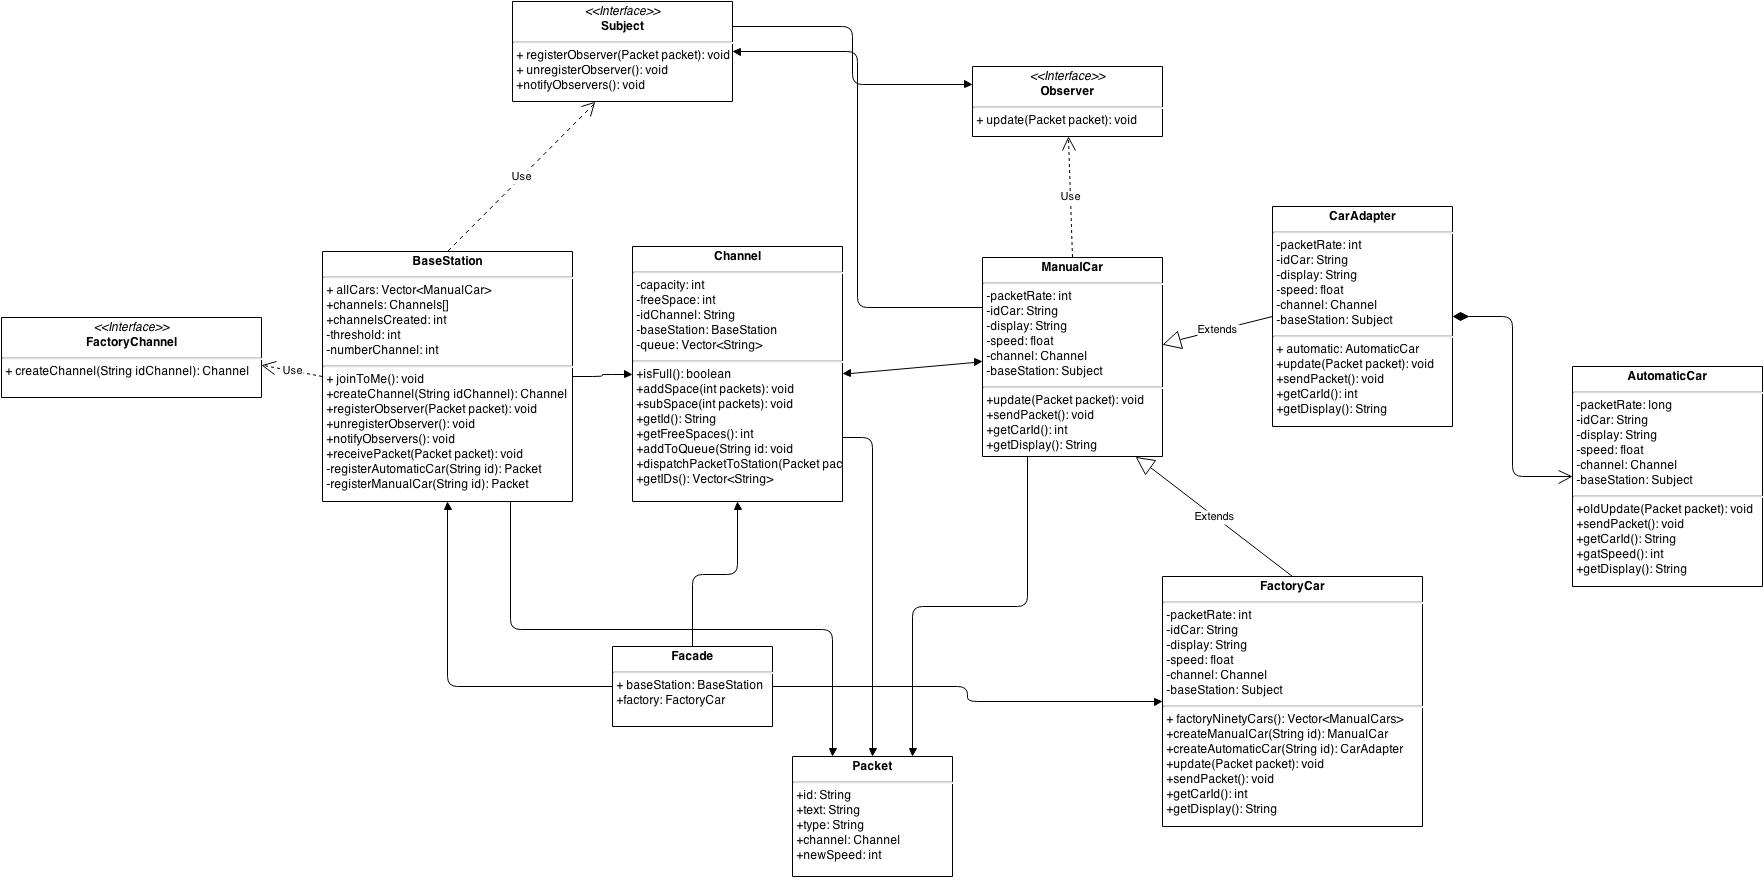
\includegraphics[scale=0.24]{class_diagram.jpg}
\caption{Diagramma delle classi}
\label{class_dig}
\end{figure}

\section{Design pattern utilizzati}

Per la creazione delle automobili abbiamo utilizzato il design pattern \textit{Factory}: la classe FactoryCar crea casualmente 90 auto, a intervalli regolari, fra automatiche e manuali. Lo stesso design pattern viene utilizzato per la creazione dei canali da parte della stazione; quest'ultima estende l'interfaccia \textit{FactoryChannel} e quando v'è necessità crea un nuovo canale. In questo modo è possibile modificare agilmente il numero di canali ed il numero di auto, interagendo con le rispettive classi.

Nella nostra modellazione utilizziamo il design pattern \textit{Observer}: le automobili osservanno la stazione, che costituisce il \textit{Subject} del pattern. La stazione ha comunque una referenza a tutte le auto in circolazione per poter inviare i messaggi necessari nella fase di setup, cioè l'invito a registrarsi come Observer presso di essa.  Non abbiamo implementato il pattern Observer fra i canali e la stazione poiché la stazione è unica.

Il pattern \textit{Adapter} viene utilizzato per adattare le auto automatiche a quelle manuali, in modo tale che il sistema, ad alto livello, conosca solo l'interfaccia di un'auto manuale (infatti gli unici costruttori invocati sono quelli di ManualCar e CarAdapter, cioè l'adattamento di un'auto automatica); ogni metodo viene adattato, in particolare il metodo \textit{oldUpdate}, metodo di AutomaticCar che in aggiunta invoca il metodo \textit{breaking}, che permette alla stazione di decrementare automaticamente la velocità della auto automatiche che superano la velocità limite espressa dal campo \textit{threshold} della stazione.

Il pattern \textit{Facade} viene utilizzato per creare un'interfaccia unica per poter interagire con l'intero sistema: la classe Facade conosce solamente la stazione e la factoryCar, che a loro volta conoscono rispettivamente i canali e le auto in circolazione; in questo modo l'interazione con il sistema può avvenire solamente tramite questa classe, nascondendo la reale implementazione degli oggetti utilizzati, in accordo con il principio di incapsulamento del paradigma ad oggetti.

\section{Simulazione del sistema}

La simulazione viene effettuata graficamente dalla classe Simulator e da alcune stampe a terminale: la classe Simulator consiste di una tabella contenente le macchine nel sistema dove per ognuna riportiamo l'identificativo, la velocità ed il messaggio sul display; i possibili messaggi sono i seguenti:
\begin{itemize}
\item \textit{Not registered}: viene visualizzato sul display dell'auto creata ma non ancora registrata presso la stazione;
\item \textit{Unregistered}: viene visualizzato sul display dell'auto quando quest'ultima viene deregistrata dal sistema;
\item \textit{Waiting for new display}: viene visualizzato sul display quando l'auto ha inviato la propria velocità ma non ha ancora ricevuto una risposta dalla stazione;
\item \textit{Good!}: viene visualizzato sul display dell'auto che rispetta la velocità limite;
\item \textit{Decrease your speed!}:  viene visualizzato sul display dell'auto che non rispetta la velocità limite;
\item \textit{Breaking}: viene visualizzato dalle auto automatiche quando la stazione rileva in esse un'eccessiva velocità e decide di decrementarla automaticamente. 
\end{itemize}

Inoltre viene riportata una finestra rappresentante la percentuale di riempimento di ciascun canale. Tutte le azione intraprese dalla stazione vengono visualizzate a terminale tramite delle stampe.

Per aggiornare i dati è necessario premere sul pulsante \textit{Refresh}.

Di seguito riportiamo un screenshot della simulazione.

\begin{figure}[htbp]
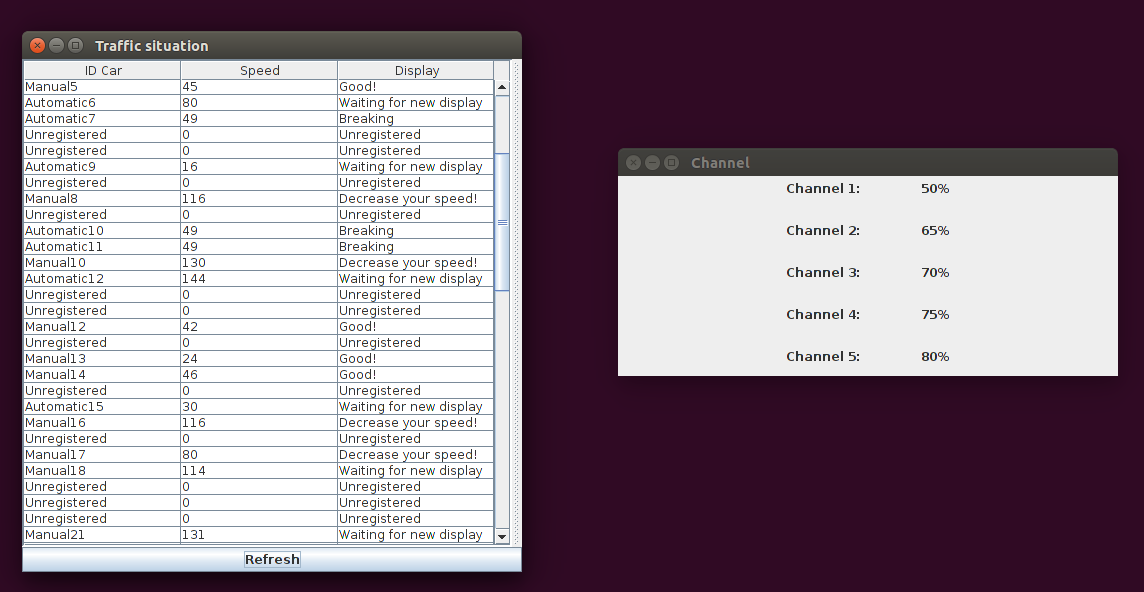
\includegraphics[scale=0.32]{screenshot.png}
\caption{Simulazione del sistema}
\label{screenshot}
\end{figure}

\end{document}
